\section{Case Study: Train Doors}
\label{sec:casestudy}

This section introduces a case study where we are
interested to verify the model correctness. In this paper, we have considered
a system that models the doors for entering or exiting of a train convoy. Such
a system is  majorly composed by three different elements: a Train Control
Management System (TCMS), a traction system and by several doors. 

The TCMS is an embedded device in charge of supervising the traction system and
the doors. Mainly, it must enable or disable the train traction and the
opening/closing of doors assuring a safe operation of the train.

Figure~\ref{fig:UMLClassDiagram-TrainDoors} depicts the UML Class diagram of
the case study. \TODO{\ldots}



\begin{figure}
  \centering
  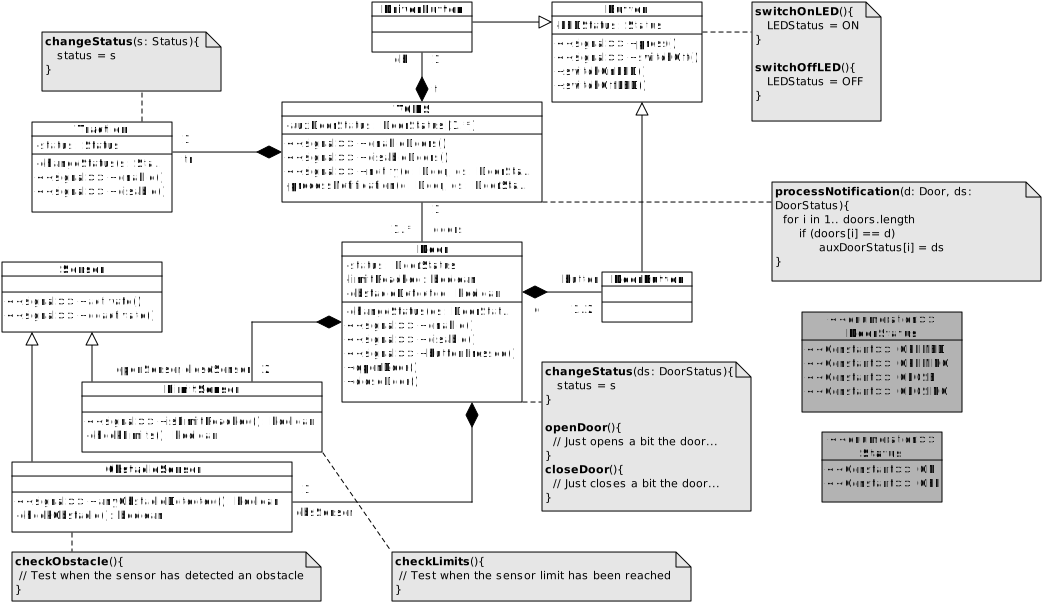
\includegraphics[width=1\columnwidth]{images/UMLClassDiagram-TrainDoors}
  \caption{UML Class diagram for the case study train doors.}
  \label{fig:UMLClassDiagram-TrainDoors}
\end{figure}


\begin{figure}
  \centering
  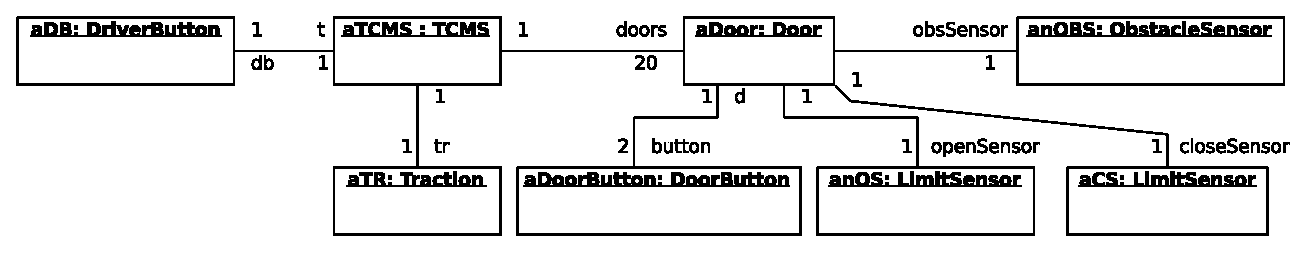
\includegraphics[width=1\columnwidth]{images/UMLObjectDiagram-TrainDoors}
  \caption{.}
  \label{fig:}
\end{figure}